\documentclass[10pt]{beamer}
\usetheme{Rochester}
\definecolor{this.blue}{RGB}{30,136,229}
\definecolor{this.red}{RGB}{204,0,0}
\definecolor{this.green}{RGB}{140,200,75}
\definecolor{this.orange}{RGB}{242,148,51}
\definecolor{this.brown}{RGB}{32,32,32}
\usecolortheme[RGB={30,136,229}]{structure}
\setbeamercolor{block title}{fg=this.blue}
%\setbeamercolor{frametitle}{fg=this.brown}
%\setbeamercolor{title}{fg=this.brown}
\setbeamercolor{block title alerted}{fg=this.red}
\setbeamercolor{block title example}{fg=this.blue}
\usepackage[]{hyperref}
\usepackage[brazil]{babel}
\usepackage{lmodern}
\usepackage{ctable}
\usepackage{amssymb,amsmath,amsfonts}
\usepackage{ifxetex,ifluatex}
\ifxetex
  \usepackage{fontspec,xltxtra,xunicode}
  \defaultfontfeatures{Mapping=tex-text,Scale=MatchLowercase}
\else
  \ifluatex
    \usepackage{fontspec}
    \defaultfontfeatures{Mapping=tex-text,Scale=MatchLowercase}
  \else
    \usepackage[utf8]{inputenc}
  \fi
\fi
% Comment these out if you don't want a slide with just the
% part/section/subsection/subsubsection title:
%\AtBeginPart{\frame{\partpage}}
%\AtBeginSection{\frame{\sectionpage}}
%\AtBeginSubsection{\frame{\subsectionpage}}
%\AtBeginSubsubsection{\frame{\subsubsectionpage}}
% new commands
\newcommand{\slidetitle}[1]{
	{\begin{center}\Huge{\textbf{\textcolor[RGB]{32,32,32}{#1}}}\end{center}}
}
\newcommand{\slidesubtitle}[1]{
	{\begin{center}\huge{\textbf{\textcolor[RGB]{51,51,51}{#1}}}\end{center}}
}
\setlength{\parindent}{0pt}
\setlength{\parskip}{6pt plus 2pt minus 1pt}
\setlength{\emergencystretch}{3em}  % prevent overfull lines
\setcounter{secnumdepth}{0}

% -- syntax highlight
\usepackage{minted}
\usemintedstyle{native}
\newcommand{\inputjscodefile}[1]{\inputminted[bgcolor=this.brown,framesep=2pt,xleftmargin=1pt,rulecolor=\color{this.brown},tabsize=3]{js}{#1}}
% -- syntax highlight

\title{WebRTC\\Real-Time Communications}
\author{Átila Camurça}

\begin{document}
\begin{frame}
\titlepage
\end{frame}

\begin{frame}\frametitle{Sumary}
\tableofcontents
\end{frame}

\section{Introdução}\label{introduuxe7uxe3o}

\begin{frame}{Introdução}

\begin{figure}[h]
    
\includegraphics[scale=0.5]{img/webrtc-logo-horiz-retro-750x140.png}
\end{figure}

\textbf{WebRTC} é um projeto livre que fornece a navegadores web e
aplicações mobile capacidade de \textbf{Real-Time Communications}
(Comunicação em tempo real) através de \emph{API}s simples.

\end{frame}

\begin{frame}{Introdução}

É uma iniciativa da W3C em conjunto com Google, Mozilla and Opera, entre
outros.

O Web Real-Time Communications Working Group foi criado para criar e
gerenciar os padrões do WebRTC.

\end{frame}

\begin{frame}{Aplicação}

Pode ser aplicado para todo tipo de plataforma que requer comunicação de
alta qualidade na web, tais como troca de \textbf{mensagens} e
transferência de \textbf{arquivos}, componentes de \textbf{áudio e
vídeo} para vídeo conferências, \textbf{comunicação e controle} de
equipamentos IoT.

\begin{figure}[h]
    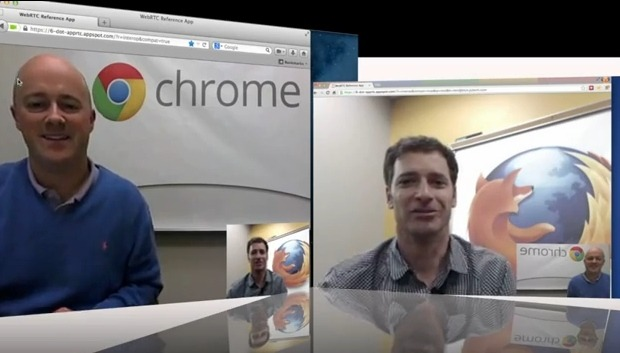
\includegraphics[scale=0.35]{img/firefox-chrome-webrtc.jpg}
\end{figure}

\end{frame}

\section{Arquitetura}\label{arquitetura}

\begin{frame}{Arquitetura}

A nível de browser:

\begin{figure}[h]
    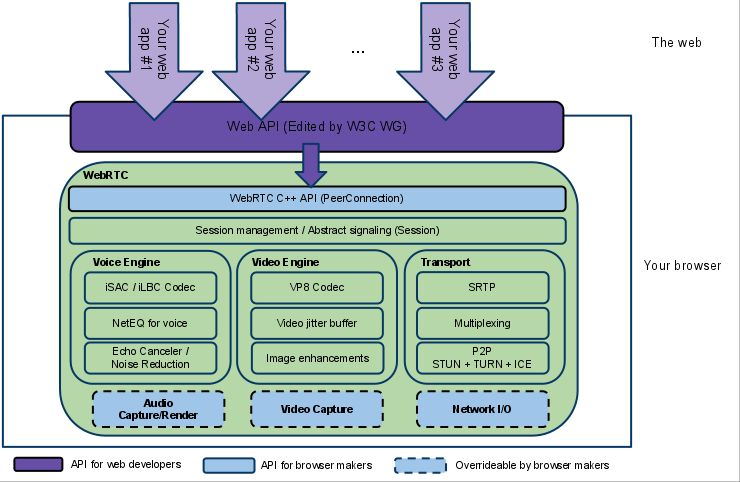
\includegraphics[scale=0.35]{img/webrtc-architecture.png}
\end{figure}

\end{frame}

\begin{frame}{Arquitetura}

WebRTC permite comunicação peer-to-peer (P2P) entre browsers

MAS ainda são necessários \textbf{servidores}:

\bigskip

\textbf{Para que clientes possam trocar metadados para coordenar a
comunicação - isto é chamado de \emph{Signaling}.}

\bigskip

\textbf{Para lidar com \emph{NAT}s (Network Address Translators) e
\emph{Firewalls}.}

\end{frame}

\begin{frame}{Arquitetura}

\begin{figure}[h]
    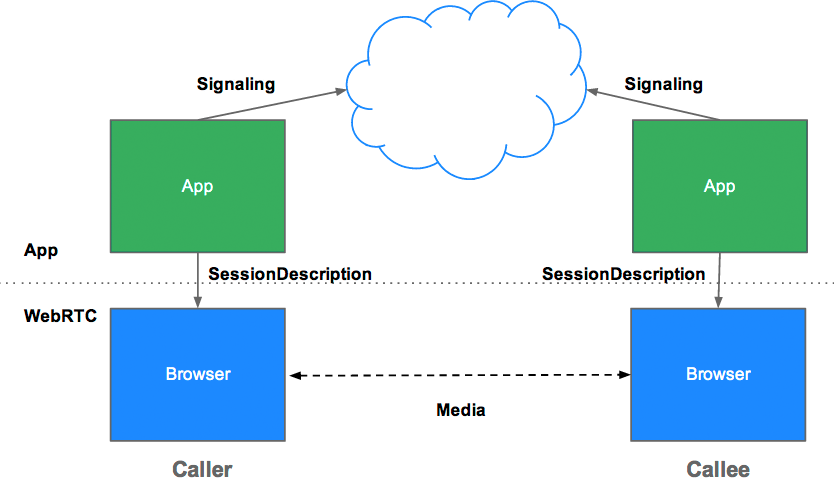
\includegraphics[scale=0.35]{img/jsep.png}
\end{figure}

\end{frame}

\begin{frame}{Arquitetura}

Para evitar redundância e maximizar a compatibilidade com tecnologias já
estabelecidas, métodos e protocolos para fazer \emph{Signaling} não
foram especificados pelos padrões do WebRTC.

A lógica por trás disso é que diferentes aplicações podem preferir
utilizar diferentes protocolos, tais como \emph{SIP} (Session Initiation
Protocol - VoIP) ou \emph{Jingle} (extensão do XMPP/Jabber - Troca de
mensagens de texto) como protocolos para fazer \emph{Signaling}.

\end{frame}


\end{document}
